% WEER talk — Hawaiʻi's Energy Future. Longer deck: broad motivation, then
% a two-frame "how the model works" section, then the talk_50min core.
% Build: build/make_slides.sh
\documentclass[11pt,aspectratio=169]{beamer}
% Shared beamer preamble — UH Mānoa / UHERO styling for the report talks.
% Loaded after \documentclass[...]{beamer} by talk_50min.tex / talk_20min.tex.
% Build: build/make_slides.sh (lualatex; DejaVu Sans is the per-glyph
% fallback so the ʻokina renders — same mechanism as the report PDF).

\usepackage{fontspec}
\directlua{luaotfload.add_fallback("slidefb",{"DejaVu Sans:mode=node;"})}
\setsansfont{texgyreheros}[Extension=.otf,UprightFont=*-regular,
  BoldFont=*-bold,ItalicFont=*-italic,BoldItalicFont=*-bolditalic,
  RawFeature={fallback=slidefb}]
\usepackage{booktabs}
\usepackage{graphicx}
\graphicspath{{../report/figures/}}

% ---- palette --------------------------------------------------------------
% uhgreen is UH Mānoa's green (from the author's teaching deck). The slate
% and brick echo the report figures' dominant colors so deck chrome and
% chart ink read as one family. Adjust hex here if matching a brand guide.
\definecolor{uhgreen}{RGB}{2,71,49}
\definecolor{uhslate}{HTML}{31708C}
\definecolor{uhbrick}{HTML}{843C39}
\definecolor{uhgray}{RGB}{200,200,200}
\definecolor{silver}{RGB}{200,200,200}

% ---- chrome ---------------------------------------------------------------
\setbeamercolor{frametitle}{fg=uhgreen}
\setbeamercolor{title}{fg=uhgreen}
\setbeamercolor{structure}{fg=uhgreen}
\setbeamercolor{local structure}{fg=uhgreen}
\setbeamercolor{section in toc}{fg=uhgreen}
\setbeamercolor{subsection in toc}{fg=uhslate}
\setbeamercolor{button}{bg=white,fg=uhslate}
\setbeamertemplate{navigation symbols}{}
\setbeamertemplate{itemize items}{--}
\setbeamercolor{itemize item}{fg=uhgreen}
\setbeamercolor{itemize subitem}{fg=uhslate}
\setbeamercolor{enumerate item}{fg=uhgreen}
\setbeamersize{text margin left=1.4em,text margin right=1.4em}
\setbeamertemplate{title page}[default][left]

% two-tone footline (green over gray) with the frame count at right
\setbeamertemplate{footline}{%
  \leavevmode%
  \hbox to \paperwidth{\hfil\scriptsize
    \color{uhgreen}\insertframenumber/\inserttotalframenumber\hspace*{2mm}}%
  \vskip2pt%
  \color{uhgreen}\rule{\paperwidth}{0.35mm}\par
  \color{uhgray}\rule{\paperwidth}{0.35mm}%
}

% transition slides: silver canvas, section title only
\newenvironment{transitionframe}{%
  \setbeamercolor{background canvas}{bg=silver}%
  \begin{frame}}{%
  \end{frame}}

% roomier itemize for content slides
\newenvironment{wideitemize}
  {\itemize\addtolength{\itemsep}{10pt}}{\enditemize}

% backup slides: keep the two-tone rules, drop the frame count
% (the count restarts after \appendix and would render as n/0)
\usepackage{appendixnumberbeamer}
\newcommand{\beginbackup}{%
  \setbeamertemplate{footline}{%
    \leavevmode\vskip8pt%
    \color{uhgreen}\rule{\paperwidth}{0.35mm}\par
    \color{uhgray}\rule{\paperwidth}{0.35mm}}}
\newcommand{\backupend}{}

% one figure, as big as the frame allows
\newcommand{\bigfig}[1]{%
  \begin{center}
    \includegraphics[width=\linewidth,height=0.82\textheight,
      keepaspectratio]{#1}
  \end{center}}


\title{\textcolor{uhgreen}{Hawaiʻi's Energy Future}}
\author{Ethan Hartley \and Michael J. Roberts}
\institute{University of Hawaiʻi at Mānoa — Economics, Sea Grant, UHERO}
\date{pre-v1.031 draft · open for comment to September 15, 2026}

\begin{document}

\begin{frame}
\maketitle
\vfill
\footnotesize All code, data, and results:
\texttt{github.com/mikejrob/oahu-electricity-future}
\end{frame}

% ---------------------------------------------------------------- motivation
\begin{frame}{Highest prices in the nation --- and the first 100\% mandate}
\begin{center}
  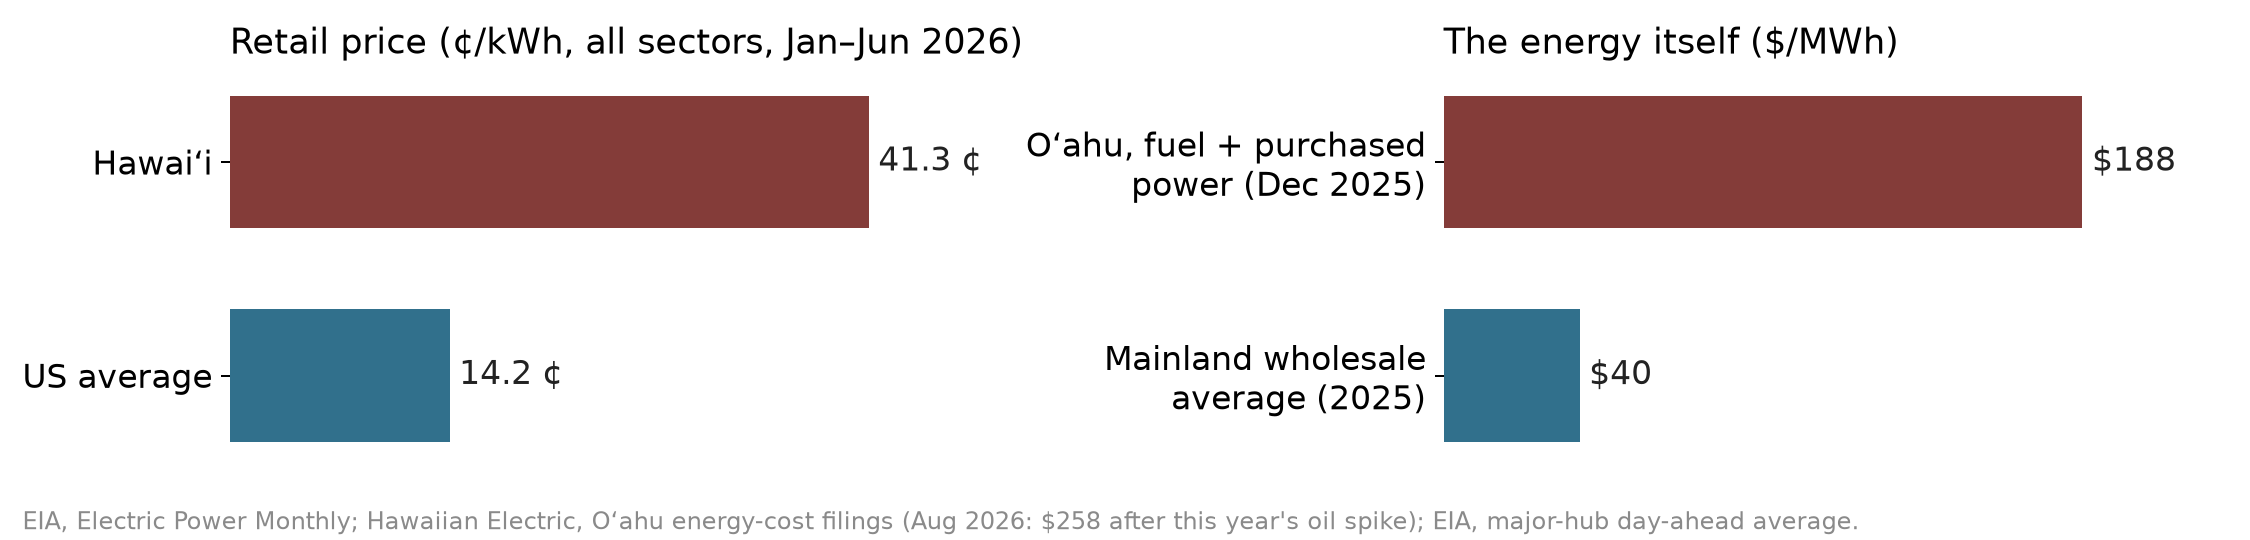
\includegraphics[width=\linewidth,height=0.62\textheight,
    keepaspectratio]{fig_weer_prices.png}
\end{center}
\vspace{-1mm}
\begin{itemize}
  \item First state to mandate 100\% renewable electricity (2015, by 2045)
  \item Ten years in, the grid is still $\sim$2/3 oil: about 33--37\%
        clean vs.\ a 43\% U.S. average
\end{itemize}
\end{frame}

\begin{frame}{Clean energy is taking over --- globally}
\bigfig{fig_weer_china.png}
\vspace{-1mm}
\begin{itemize}
  \item Spot LNG roughly doubled since the Hormuz closure
        (\$11--13 $\to$ \$22--23/MMBtu); diesel cracks at all-time records
  \item Electric vehicles: $\sim$2/3 of recent new-car sales in China,
        $\sim$2/3 of India's three-wheeler sales
\end{itemize}
\end{frame}

\begin{frame}{The U.S. bottleneck: connecting to the grid}
\begin{center}
  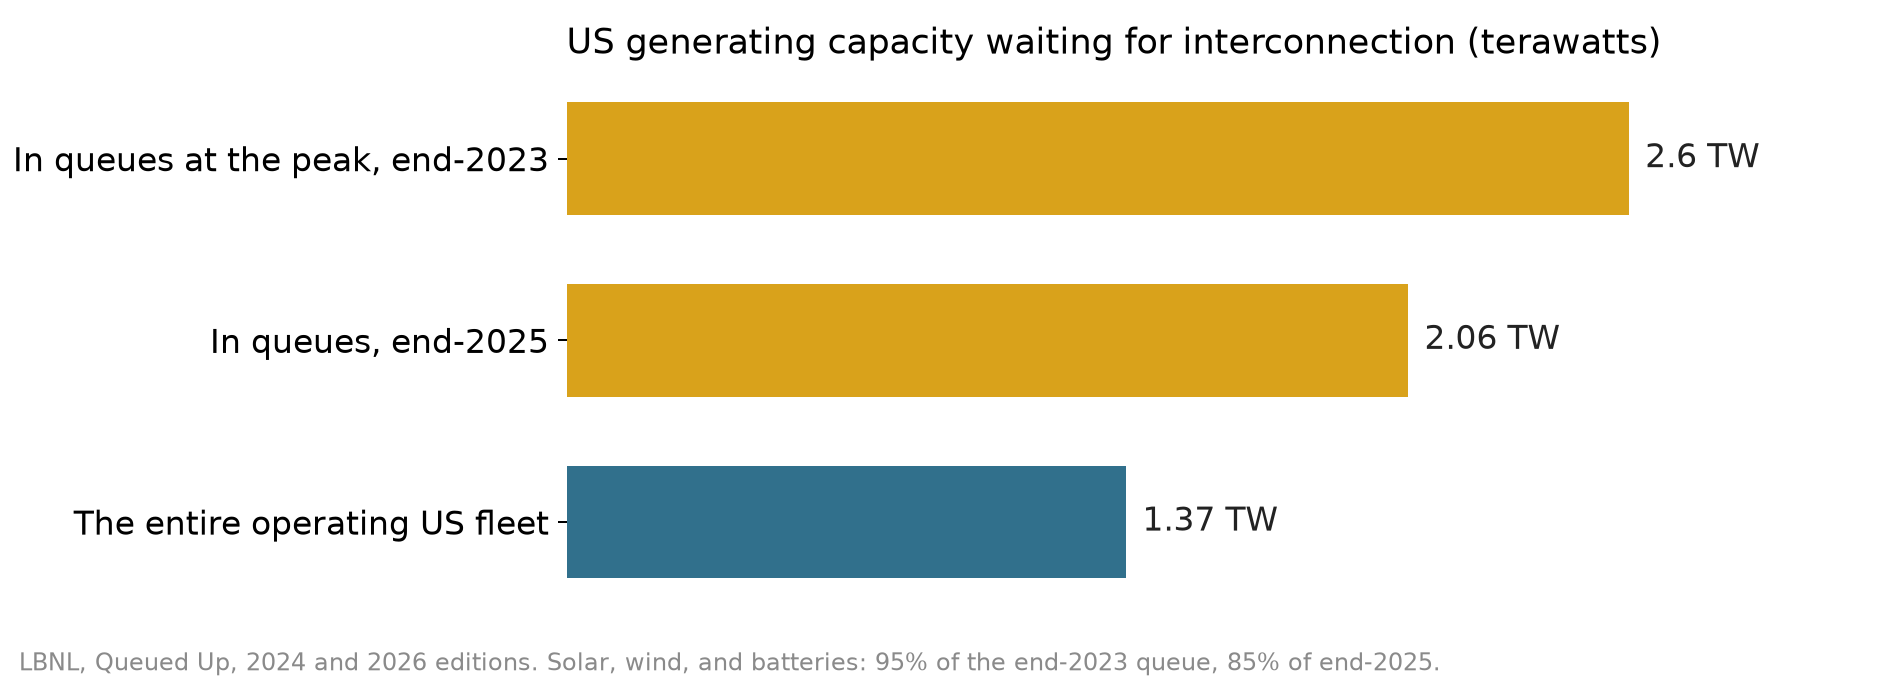
\includegraphics[width=\linewidth,height=0.52\textheight,
    keepaspectratio]{fig_weer_queue.png}
\end{center}
\vspace{-2mm}
\begin{itemize}
  \item Median wait: 5+ years for projects finished in 2025, under 2 in
        2008; of capacity queued 2000--2020, 13\% was operating by end-2025
  \item Panels are $\sim$25\% of a U.S. utility solar project
        ($\sim$16\% with storage); field labor $\sim$22\% and design,
        overhead \& other soft costs $\sim$16\% of the total (NREL 2025)
  \item IRENA 2025: U.S. installed cost 2.2$\times$ China's (\$1{,}180
        vs.\ \$533/kW); China is cheaper on 13 of 16 components, and
        the panel gap is one of the smaller ones
\end{itemize}
\end{frame}

\begin{frame}{Hawaiʻi has the problem in its sharpest form}
\begin{wideitemize}
  \item \textbf{Rooftop solar}: the nation's largest share, $\sim$18\% of
        sales (California next, $\sim$13\%) --- yet daytime exports earn
        10--13.5~\textcent\ by tranche, roughly half the filed avoided
        energy cost ($\sim$24~\textcent) and under a third of retail
  \item \textbf{Utility solar}: highest prices in the country
        ($\sim$2$\times$ mainland) --- and interconnection as slow as the
        mainland's, without the queue
  \item \textbf{The response on offer}: new oil and LNG plants
\end{wideitemize}
\vspace{0.4cm}
\begin{center}
  {\Large \textcolor{uhgreen}{The crux: make it easy to connect to the
   grid and sell power at a fair price.}}
\end{center}
\end{frame}

% ---------------------------------------------------------------- setting
\begin{frame}{Three decisions are on the table now}
\begin{wideitemize}
  \item \textbf{Waiau Repower} — six oil-fired turbines, approved March 2026
  \item \textbf{JERA proposal} — \$2B, 500 MW plant + LNG import terminal
  \item \textbf{Utility-scale solar} — procurement has stalled; land rules
        \emph{may} bind
\end{wideitemize}
\vspace{0.4cm}
Each choice locks in decades.
\end{frame}

\begin{frame}{What we built}
\begin{wideitemize}
  \item Open capacity-expansion model of Oʻahu, 2027--2050 --- built on
        Switch (Fripp), updated and extended
  \item Hourly operations: unit commitment, reserves, storage, EVs
  \item 500+ solved scenarios: oil prices, solar costs, land rules,
        LNG, geothermal
  \item Everything public --- inputs, code, results, an interactive
        explorer; anyone can replicate it or test their own scenarios
\end{wideitemize}
\end{frame}

% ---------------------------------------------------------------- how it works
\begin{transitionframe}
  \begin{center}{\Huge \textcolor{black}{How the model works}}\end{center}
\end{transitionframe}

\begin{frame}{The model in words}
\begin{wideitemize}
  \item \textbf{Decides}: what to build and when --- solar, wind,
        batteries, geothermal, plants --- and how to run everything,
        hour by hour
  \item \textbf{Objective}: lowest total cost of electricity through 2050
        (capital, fuel, and operations)
  \item \textbf{Always}: demand met every hour; reserves held for the
        largest unit running, plus swings in wind and solar
  \item \textbf{Limits}: land for solar, build schedules, existing plants
        and contracts, 100\% renewable by 2045
  \item \textbf{Flexibility}: batteries, 50\% of EV charging, and hydrogen
        production scheduled to the cheapest hours
\end{wideitemize}
\end{frame}

\begin{frame}{Each model year: 13 sample days, weighted}
\begin{center}
  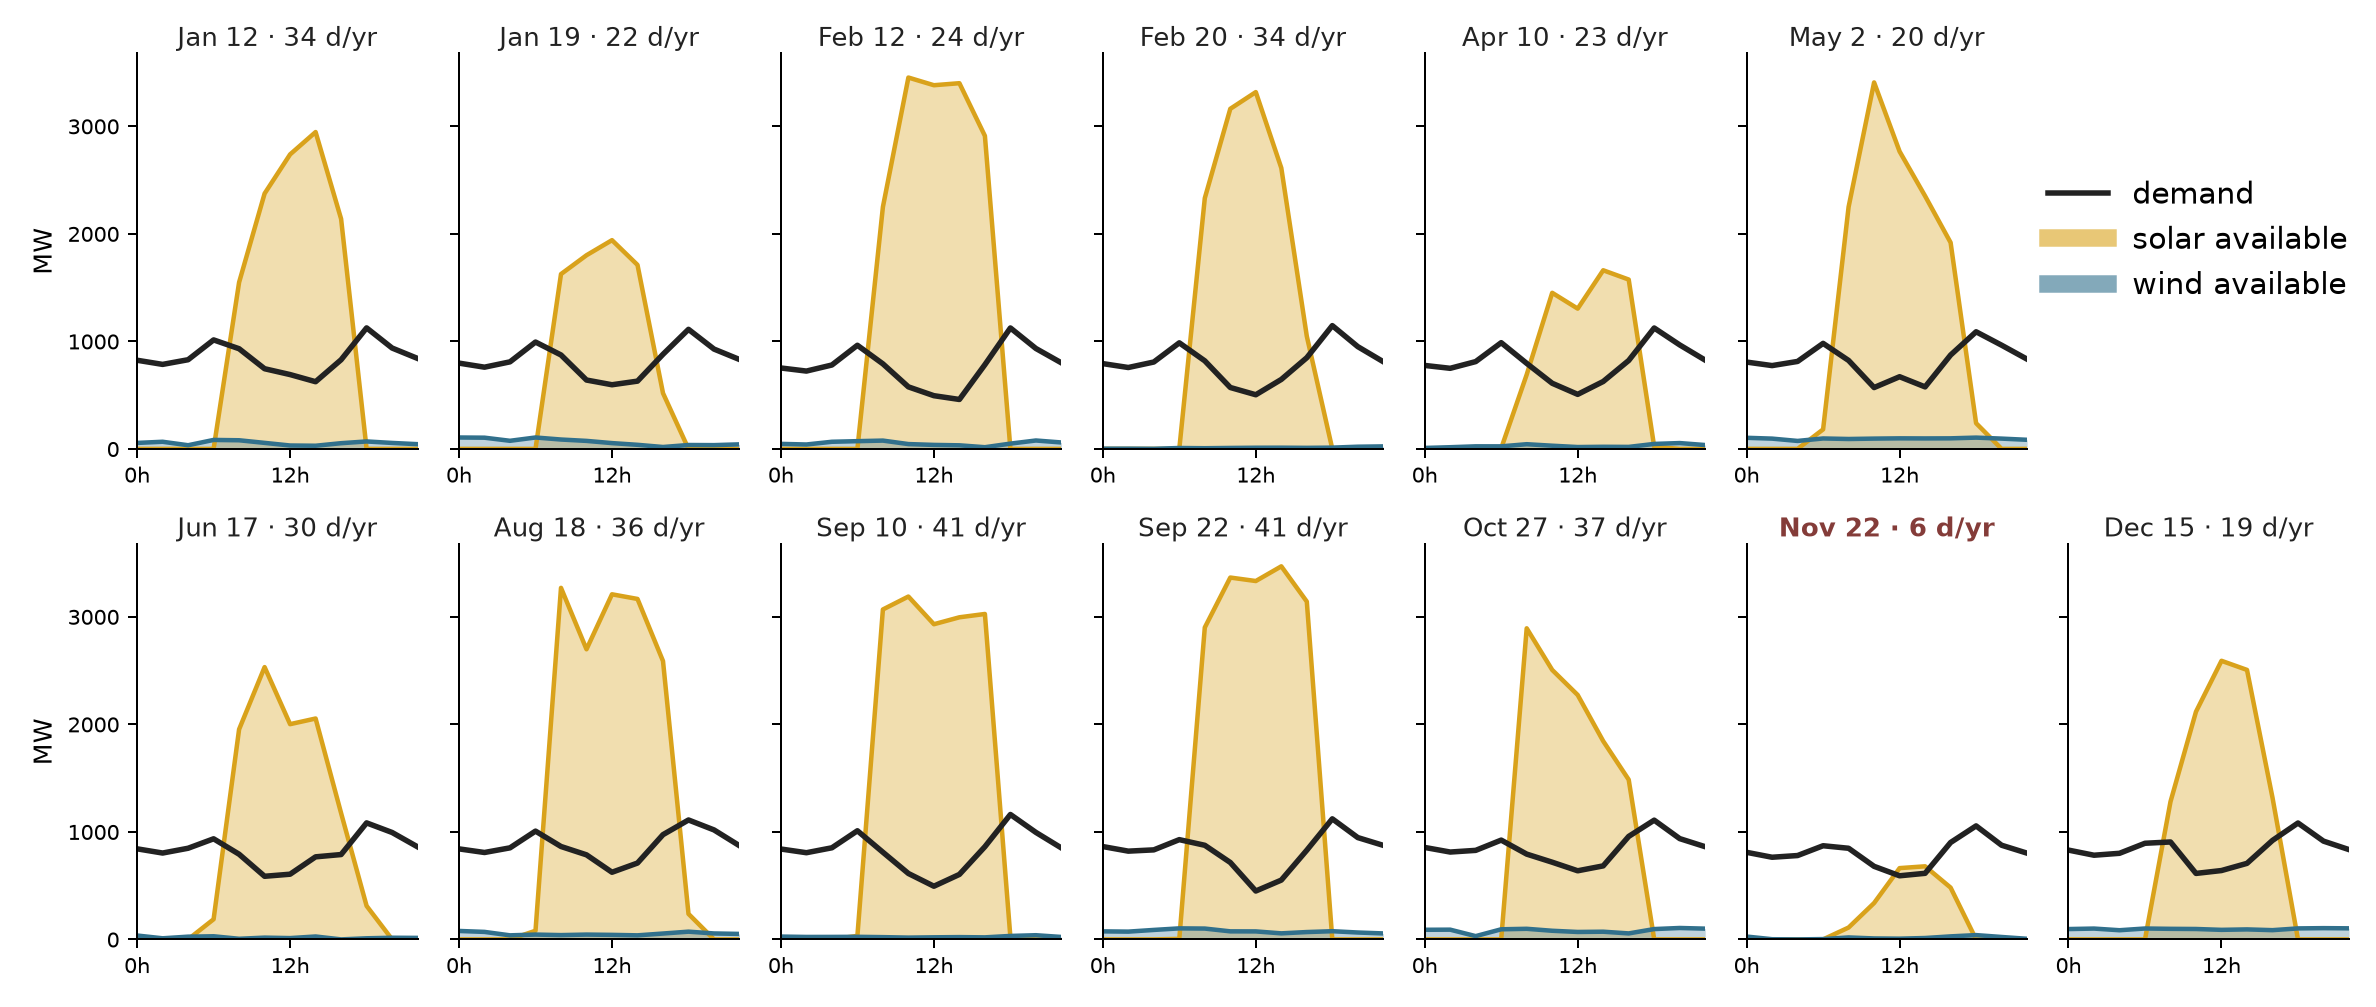
\includegraphics[width=\linewidth,height=0.74\textheight,
    keepaspectratio]{fig_sample_days_2045.png}
\end{center}
\vspace{-2mm}
{\footnotesize 2045, no-new-plant base case. Solar and wind at full
availability from the capacity the model built; demand is net of rooftop
solar and excludes flexible EV and hydrogen loads, which the model
schedules. \textcolor{uhbrick}{Nov 22}: the record's hardest day.}
\end{frame}

\begin{frame}{The scenario space}
\bigfig{fig_scenario_map.png}
\end{frame}

% ---------------------------------------------------------------- land
\begin{transitionframe}
  \begin{center}{\Huge \textcolor{black}{Solar and land}}\end{center}
\end{transitionframe}

\begin{frame}{Plausibly available land, and what the model uses}
\begin{columns}[c]
  \begin{column}{0.58\textwidth}
    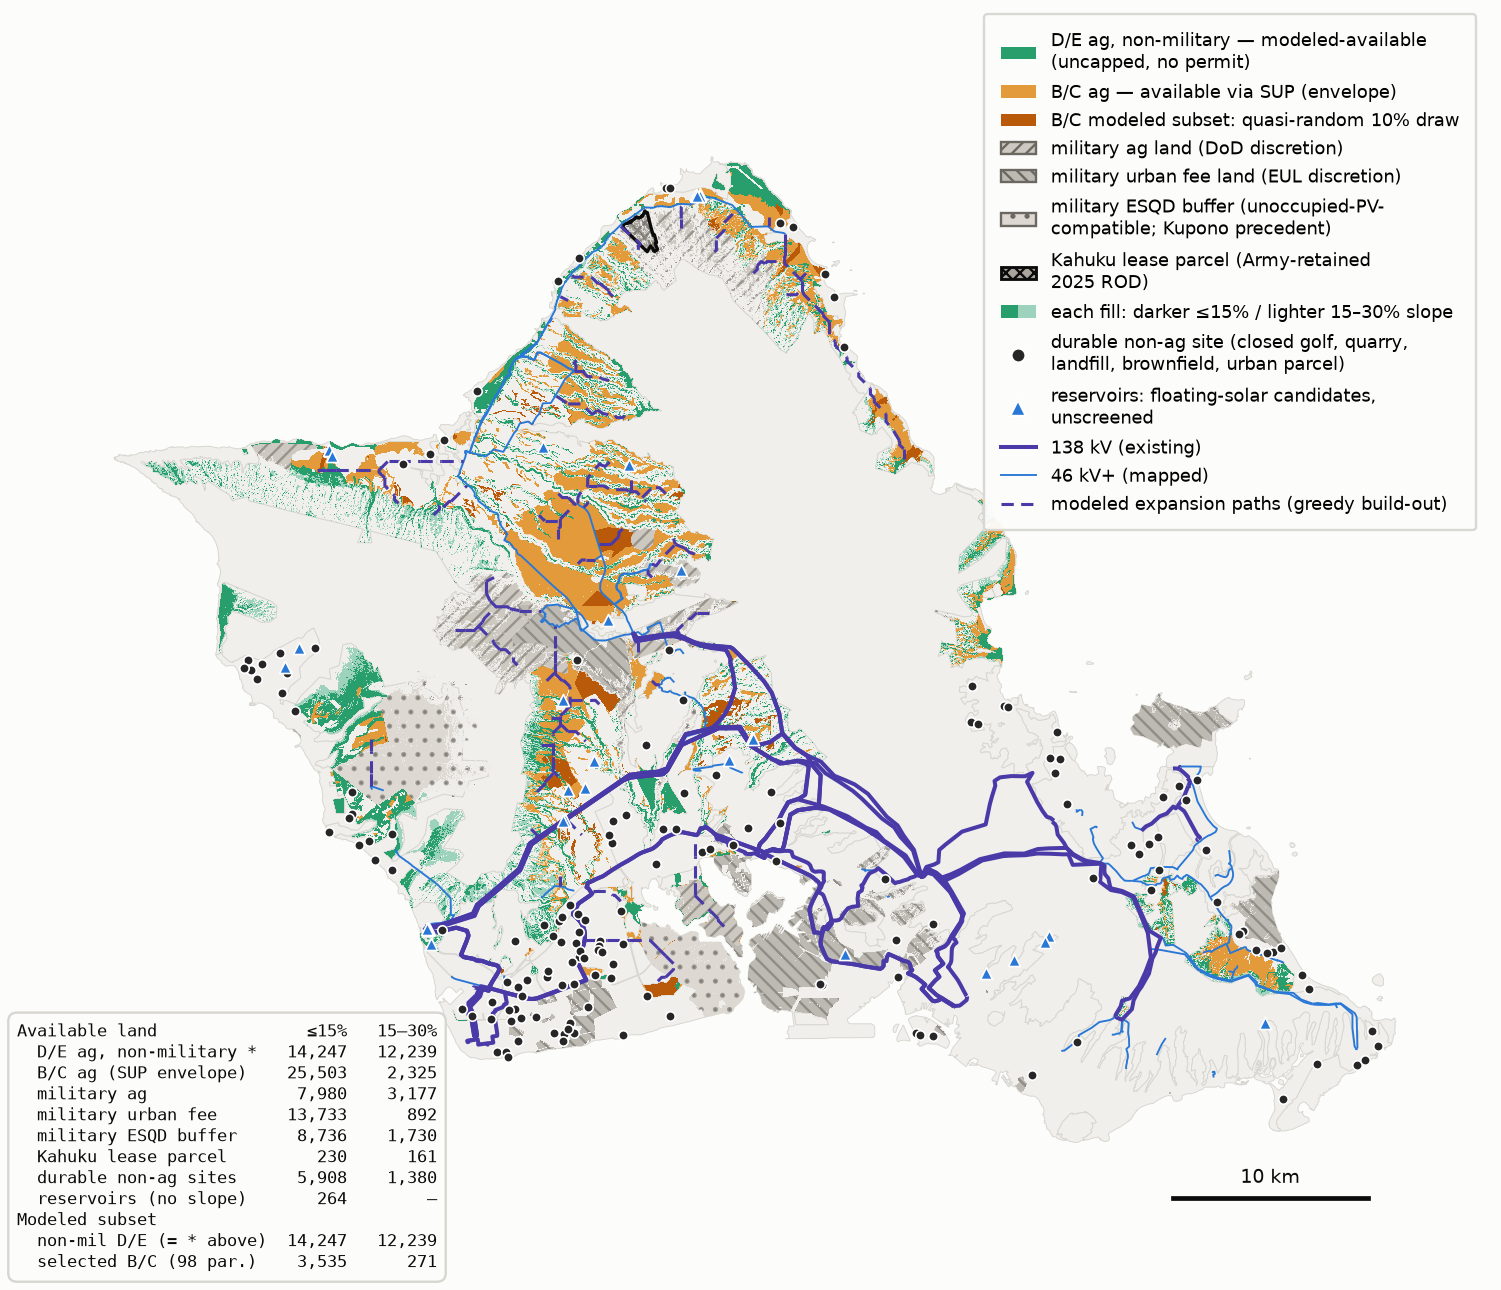
\includegraphics[height=0.85\textheight,
      keepaspectratio]{fig_2_3_available_land_map_slide.png}
  \end{column}
  \begin{column}{0.4\textwidth}
    \small
    Each fill has two shades: darker $\le$15\% slope, lighter the
    15--30\% increment.\\[0.7em]
    The modeled subset is non-military D/E agricultural land (green)
    plus a quasi-random 10\% draw of B/C (dark orange).\\[0.7em]
    Military land is shown by tenure --- available at DoD discretion,
    not in the modeled subset.\\[0.7em]
    No grid-distance filter; published near-grid figures are smaller.
  \end{column}
\end{columns}
\end{frame}

\begin{frame}{How much land, and when}
\bigfig{fig_2_1_land_timing.png}
\end{frame}

\begin{frame}{Rooftops change the land question}
\begin{wideitemize}
  \item Measured potential: about 4{,}000 MW on existing structures
  \item Three adoption paths: $\sim$1{,}000 / 1{,}600 / 2{,}100 MW by 2050
  \item Fast rooftop growth: utility solar falls from 4{,}100 to
        3{,}000 MW; land toward 15{,}000 acres
  \item What unlocks it: paying fair value for exports (Section 2.7)
\end{wideitemize}
\end{frame}

\begin{frame}{Hawaiʻi pays a large, unexplained solar premium}
\begin{center}
  {\LARGE Utility solar here: \textcolor{uhbrick}{1.4 to 2.2+$\times$}
   mainland cost}
\end{center}
\vspace{0.4cm}
\begin{wideitemize}
  \item Physical conditions explain only part
  \item 2018-era contracts (Phase 1, Kauaʻi) came in \emph{below} 1.8$\times$
  \item Recent Oʻahu repricings anchor the top of the range
\end{wideitemize}
\end{frame}

\begin{frame}{The premium is in the process, not the hardware}
\begin{center}
\renewcommand{\arraystretch}{1.3}
\begin{tabular}{lcc}
\toprule
Utility solar + storage & Hawaiʻi & Mainland \\
\midrule
Contracts of 2018--20         & 7.7 \textcent & 3.1 \textcent \\
Contracts of 2024--26         & 19.5 \textcent & 6.5 \textcent \\
\midrule
The same global shock added   & \textcolor{uhbrick}{$+$12 \textcent}
                              & $+$2.5--3.5 \textcent \\
\bottomrule
\end{tabular}
\end{center}
\vspace{0.2cm}
{\footnotesize Levelized 2024\textcent/kWh, matched configuration. The
12\textcent\ is Mahi --- the \emph{same project}, repriced. Meanwhile
grid-battery packs fell \textbf{45\% in 2025 alone}, to \$70/kWh
(BloombergNEF).}
\vspace{0.2cm}
\begin{itemize}
  \item \textbf{Rooftop}: modest. Tesla's by-state pricing (8 kW+):
        Hawaiʻi \$2.90/W, between California (\$2.83) and New York
        (\$2.98)
  \item \textbf{Utility-scale}: \textcolor{uhbrick}{2--3$\times$}.
        Similar panels, labor, and land --- most of the difference
        appears to be soft costs
  \item \textbf{One mechanism}: a PPA fixes its price in nominal dollars
        at award, and award-to-operation runs \textbf{4--7 years} on
        Oʻahu. Inflation eats the award, so developers bid high,
        reprice, or walk
\end{itemize}
\end{frame}

% ---------------------------------------------------------------- JERA
\begin{transitionframe}
  \begin{center}{\Huge \textcolor{black}{Does a new fuel plant pay?}}\end{center}
\end{transitionframe}

\begin{frame}{No proposed plant beats building no plant}
\bigfig{fig_ES1_jera_bracket.png}
\end{frame}

\begin{frame}{What the system builds instead}
\bigfig{fig_genmix.png}
\end{frame}

\begin{frame}{The verdict survives expensive solar}
\bigfig{fig_4_2_solar_sensitivity.png}
\end{frame}

\begin{frame}{\ldots and every oil price}
\bigfig{fig_4_3_oil_solar_matrix.png}
\end{frame}

\begin{frame}{If LNG comes, existing plants beat new ones}
\begin{center}
\renewcommand{\arraystretch}{1.4}
\begin{tabular}{lr}
\toprule
LNG configuration (vs.\ no new plant) & $\Delta$ cost \\
\midrule
New JERA plant (midpoint)            & \textcolor{uhbrick}{$+\$0.7$--$1.6$B} \\
Convert Kalaeloa alone               & \textcolor{uhgreen}{$-\$0.4$B} \\
\ \ + Kahe 5\,\&\,6, CIP turbine     & \textcolor{uhgreen}{$-\$1.1$B} \\
\bottomrule
\end{tabular}
\end{center}
\vspace{0.3cm}
Same fuel savings, no construction. Conversion budgets: $\sim$\$1{,}800/kW
before the case breaks.

\vspace{0.2cm}
{\small And the LNG itself is a bet: a long-term \emph{quantity} contract,
likely with a price floor. We model \$11.4/MMBtu delivered --- today's
spot is about \textcolor{uhbrick}{twice} that.}
\end{frame}

\begin{frame}{LNG's climate case hangs on methane leakage}
\bigfig{fig_4_1_emissions.png}
\end{frame}

\begin{frame}{The leakage arithmetic}
\begin{center}
  {\LARGE Greenhouse advantage gone above
   \textcolor{uhbrick}{$\sim$0.9\%} supply-chain leakage}
\end{center}
\vspace{0.4cm}
\begin{wideitemize}
  \item (100-year basis; $\sim$0.3\% on a 20-year basis)
  \item Measured U.S. supply-chain rates sit well above both thresholds
\end{wideitemize}
\end{frame}

% ---------------------------------------------------------------- plans
\begin{transitionframe}
  \begin{center}{\Huge \textcolor{black}{The plans on file}}\end{center}
\end{transitionframe}

\begin{frame}{Our least-cost paths vs.\ HECO's IGP and HSEO's study}
\bigfig{fig_4_4_plan_comparison.png}
\end{frame}

\begin{frame}{Every plan, priced on one ruler}
\bigfig{fig_4_5_plan_price_tags.png}
\end{frame}

% ---------------------------------------------------------------- EGS
\begin{transitionframe}
  \begin{center}{\Huge \textcolor{black}{Enhanced geothermal}}\end{center}
\end{transitionframe}

\begin{frame}{A small resource with outsized value}
\begin{wideitemize}
  \item First resource screen: $\sim$100 MW identified on Oʻahu
  \item The model builds all of it in the base case
  \item Blocking it costs \textcolor{uhbrick}{+\$0.6B}; at optimistic
        drilling costs the saving reaches \textcolor{uhgreen}{$\sim$\$1.0B}
  \item 100 MW displaces $\sim$400 MW of solar land
  \item The resource at depth is unmeasured --- could be far larger
\end{wideitemize}
\end{frame}

% ---------------------------------------------------------------- reliability
\begin{transitionframe}
  \begin{center}{\Huge \textcolor{black}{Reliability}}\end{center}
\end{transitionframe}

\begin{frame}{The hard day is not the peak day}
\bigfig{fig_5_1_reliability_days.png}
\end{frame}

\begin{frame}{Resource adequacy: covered with room to spare}
\bigfig{fig_reserve_cushion.png}
\end{frame}

\begin{frame}{Resilience changes on a renewable grid}
\begin{wideitemize}
  \item Firm plants cover the daily-average net load
        (\textcolor{uhslate}{$\sim$610 MW} in 2035); batteries carry
        energy to the evening peak (\textcolor{uhslate}{$\sim$1,270 MW})
  \item Generation comes in thousands of pieces --- the main risk
        becomes island-wide, multi-day, forecastable weather
  \item Two units out at a thin hour, at the filed 10\% failure rate:
        \textcolor{uhgreen}{$\sim$6 h/yr} --- conventional
        standards run 2--8 h/yr
  \item The real tail: correlated failures and storage depth
        (a 16-day low-wind run is on record) --- v2 tests both
\end{wideitemize}
\end{frame}

\begin{frame}{The Waiau Repower fails its own cost test}
\begin{wideitemize}
  \item Adds \textcolor{uhbrick}{+\$1.4B} to system cost on every oil path
  \item Runs at 51\% in 2030, under 32\% by the late 2030s,
        $\sim$0 from 2045
  \item A modern combined cycle delivers the same firm capacity at
        $\sim$1/3 less per kW
  \item PUC cost cap: \$220--310M of the bill lands on shareholders
\end{wideitemize}
\end{frame}

% ---------------------------------------------------------------- reform
\begin{transitionframe}
  \begin{center}{\Huge \textcolor{black}{What reform unlocks}}\end{center}
\end{transitionframe}

\begin{frame}{Three levers, no new technology required}
\begin{wideitemize}
  \item \textbf{Land}: state siting rules exclude most of the island's
        flat, cleared, transmission-adjacent land
  \item \textbf{Procurement}: independent bid evaluation, standard
        contracts, published queues
  \item \textbf{Rooftops}: pay fair value for exported power
\end{wideitemize}
\vspace{0.4cm}
The savings at stake dwarf every supply-side proposal on the table.
\end{frame}

\begin{frame}{The deeper reform: retail wheeling}
\begin{wideitemize}
  \item The Legislature has mandated retail wheeling --- \emph{how} is
        the open question
  \item Our proposal (Schedule RWS, in preparation): sellers and large
        buyers settle at \textbf{locational marginal prices}; the
        utility keeps the wires
  \item Ten-day provisional interconnection replaces the RFP gauntlet
  \item Real-time prices unlock demand flexibility
        (Imelda, Fripp \& Roberts 2024, \emph{AEJ: Policy})
  \item Self-funding: a transition fund captures part of today's
        oil-priced margins
\end{wideitemize}
\end{frame}

\begin{frame}{Even if solar stays expensive here, the answer holds}
\bigfig{fig_2_4_high_solar_cost_pathways.png}
\end{frame}

% ---------------------------------------------------------------- oil risk
\begin{transitionframe}
  \begin{center}{\Huge \textcolor{black}{The oil bet}}\end{center}
\end{transitionframe}

\begin{frame}{Four oil futures, priced from markets}
\bigfig{fig_A14_oil_cases.png}
\end{frame}

\begin{frame}{Demand is falling in 2026 --- without the recession that
  always came before}
\bigfig{fig_8_1_decline_vs_gdp_usrec.png}
\end{frame}

% ---------------------------------------------------------------- close
\begin{transitionframe}
  \begin{center}{\Huge \textcolor{black}{Takeaways}}\end{center}
\end{transitionframe}

\begin{frame}{Takeaways}
\begin{wideitemize}
  \item \textbf{No proposed fuel plant pays for itself} --- not JERA's,
        not the Waiau Repower, under any oil or solar price we can defend
  \item \textbf{Solar + storage + existing plants} is the robust
        least-cost core; geothermal sweetens it
  \item \textbf{The binding constraints are rules, not resources} ---
        land, procurement, and rooftop compensation
\end{wideitemize}
\end{frame}

\begin{frame}{Kick the tires}
\begin{center}
  {\Large \texttt{github.com/mikejrob/oahu-electricity-future}}
\end{center}
\vspace{0.3cm}
\begin{wideitemize}
  \item Full report, all inputs, all 500+ solved scenarios
  \item Interactive explorer --- every figure, every configuration
  \item Comments to September 15, 2026; we answer publicly
\end{wideitemize}
\end{frame}

% ---------------------------------------------------------------- backup
\appendix
\beginbackup
\begin{transitionframe}
  \begin{center}{\Huge \textcolor{black}{Backup}}\end{center}
\end{transitionframe}

\begin{frame}{System cost by trajectory and oil price (Table ES.1)}
\begin{center}
\small
\renewcommand{\arraystretch}{1.25}
\begin{tabular}{lcccc}
\toprule
 & Market 10th & Brent futures & EIA ref. & Market 90th \\
\midrule
No new fuel plant       & 21.2 & 24.3 & 25.8 & 27.3 \\
Modern LSFO plant       & +0.7 & +0.5 & +0.4 & +0.6 \\
JERA LNG (midpoint)     & +1.6 & +0.7 & +0.8 & +1.2 \\
Waiau Repower           & +1.4 & +1.4 & +1.4 & +1.5 \\
Waiau + JERA            & +3.1 & +2.1 & +2.2 & +2.7 \\
\bottomrule
\end{tabular}

\vspace{0.3cm}
Billions of 2024\$, present value 2027--2050, 3\% real.
\end{center}
\end{frame}

\begin{frame}{Method guardrails}
\begin{wideitemize}
  \item 0.1\% optimization tolerance; dominance checks across 698
        scenario pairs gate every release
  \item 13 sample days per period include the record's hardest day
        (Nov.\ 22, 2008: low sun, weak trades)
  \item Reserves every hour: the largest unit online, plus regulation
        that grows with solar and wind output
  \item Conservative for renewables: no inter-day storage, no real-time
        pricing, distributed value uncredited
\end{wideitemize}
\end{frame}

\begin{frame}{Since the draft: Kalaeloa signed for 30 more years}
\begin{wideitemize}
  \item New PPA signed July 27, 2026 (pending PUC approval)
  \item 208 MW firm, biofuel-capable repowering, $\sim$2033--2063
  \item Capacity charge \emph{fell} \$7/kW-yr --- firm capacity without
        new construction keeps beating new plants
\end{wideitemize}
\end{frame}

\backupend
\end{document}
